\chapter{基礎知識}
\cout{
本章では,本論文で扱うProgrammable Microfluidic Device(PMD)というバイオチップの基礎知識についての説明をする.
まず,PMDのアーキテクチャについて説明する.
そして,PMDのアーキテクチャの欠点についても説明する.
最後に,既存手法として,PMDのアーキテクチャの欠点に対応したPMD上での混合手順の生成手法
No Transport Mixing(NTM)について簡単に説明する.}
\section{PMD}
\cout{この節では,PMDというデバイスがどういったアーキテクチャを持つかを説明する.}
\subsection{PMDのアーキテクチャ}
%PMDとはどういうデバイスか説明を書く.
\cout{
PMDの顕微鏡写真を図~\ref{fig:micrograph}に示した~\cite{1}.
図~\ref{fig:micrograph}において,赤黒く見えるのはバルブという部品で,バルブによって囲まれていて青い線の交点と重なっている領域はセルと呼ばれる.
バルブは開閉操作を行うことが可能である.
図~\ref{fig:mixing}では,PMDに流し込まれた試薬が混合される様子を表している~\cite{4}.
図~\ref{fig:mixing}の(a)\~(b)は,圧力をかけられることで試薬が入力ポートからPMDの内部へと流入する様子を表している.
図~\ref{fig:mixing}の(c)は,バルブの開閉の制御によって,ミキサーと呼ばれるセルが円環状に繋げられた流路が生成される様子を表している.
ミキサー内のバルブの開閉を行うことにより,ミキサー内の液滴の混合が行われる.
そして,液滴の混合が行われると,ミキサー内のどのセルにおいても格納している液滴の濃度は等しくなる.
}
\begin{figure}[tbp]
 \centering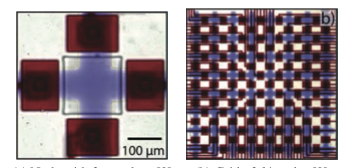
\includegraphics[scale=1.0]{img/PMDMicrograph.pdf}
 \caption{PMDの顕微鏡写真}\label{fig:micrograph}
\end{figure}
\begin{figure}[tbp]
 \centering\includegraphics[scale=1.3]{img/PMDMixing.pdf}
 \caption{PMD上に流し込まれた2種類の試薬が混合される様子}\label{fig:mixing}
\end{figure}
\subsection{PMDにおけるセル間の液滴の移動}
%既存手法の説明への前提知識として,PMDにおいてセル間での液滴の移動操作は原則不可能であるということを説明する.
\cout{PMDにおいて,セル間での液滴の移動操作は原則的に不可能であることが知られている.
それは,fluid segmentationと呼ばれる,セル間の経路上において運んでいる液滴が散り散りになる現象が起きるからだ~\cite{FU2015343}.
したがって,PMDで試薬合成を行うためには,セル間での液滴の移動なしで液滴の混合を行っていく必要がある.
}
\section{{2×2ミキサーを用いた液滴移動の\bout{ない}混合手順の生成}}
%セル間の液滴の移動操作を必要としない試薬混合手法NTM(No Transport Mixing)の説明をする.
%その後,既存の希釈木のNTMでのPMDへのマッピング手法を説明する.
\cout{
    Choudharyらは,セル間での移動なしで試薬合成を行うことができる試薬の混合手順の生成手法NTMを提案した~\cite{4}.
    図~\ref{fig:ntmresult}はNTMの入出力データを表している~\cite{4}.
}
\begin{figure}[tbp]
 \centering\includegraphics[scale=1.5]{img/NTMResult.pdf}
    \caption{NTMの入出力データ}\label{fig:ntmresult}
\end{figure}


